\documentclass[11pt]{article}

\def\baselinestretch{1}
\usepackage{times}
\usepackage{titlesec}
\usepackage{fancyhdr}  % for displaying head/foot meta info 
\usepackage{pagecounting}
\usepackage{color}
\usepackage[yyyymmdd,hhmmss]{datetime}  % for using currenttime command 
\usepackage{hyperref}
\usepackage{lastpage}
\usepackage{lipsum}
\usepackage{graphicx}
\usepackage{caption}
\usepackage{subcaption}

\graphicspath{ {../images/rubis/} {../images/gbmperf_charts/} }

\newcommand\bb[1]{\mbox{\em #1}}
\newcommand{\eat}[1]{}
\newcommand{\hsp}{\hspace*{\parindent}}
\definecolor{gray}{rgb}{0.4,0.4,0.4}


\titleformat{\section}{\vspace{- 0.5 \baselineskip}\normalfont\fontsize{12}{12}\bfseries}{\thesection}{1em}{}
\titleformat{\subsection}{\vspace{- 0.5 \baselineskip}\normalfont\fontsize{11}{11}\bfseries}{\thesubsection}{1em}{}

\begin{document}

\renewcommand{\headrulewidth}{0pt} 
\renewcommand{\footrulewidth}{0pt} 
\pagestyle{fancy}
\cfoot{}
\lhead{}
\rhead{}
\rfoot{\itshape\textcolor{gray}{Page \thepage\ of \pageref{LastPage}}}
\lfoot{\itshape\textcolor{gray}{CS525T Cloud Computing Paper Review}}

%%% Fill in the paper information %%%
\begin{center}
{\LARGE \bf Midterm Review: Comparison Between Virtual Machines and Containers for Cloud End Users} \\
{\normalsize \emph{Heshan Perera, Michael Ludwig}}\\

\end{center}

\section{Project Log}

So far our project is on track, with some changes to our selection of benchmarks. We tried moving forward with MLPerf, however the implementations are all written for GPUs. Although both AWS EC2 and ECS support instances with GPUs, they are prohibitively expensive to work with while using the AWS Educate accounts. Instead, we ended up using a benchmark called gbmperf [1], which trains a model using three different gradient boosting libraries. This gives a realistic workload for standard ML use cases. We were able to move forward with the RUBiS benchmark as we had planned. 

An additional step we would like to add to our project is using sysbench or another similar tool to benchmark specific resources in order to see which, if any, have different performance. This will help explain any disparities in the other benchmark results.

\section{Complete Work}

For our first phase we had selected two benchmarks, gbmperf and RUBiS. RUBiS is an open-source auction site prototype modeled after eBay.com developed by Rice University. It has been widely used as a benchmark in the area of network research. The workload generated for RUBiS is a continuous stream of HTTP requests to an auction site for a specified period of time. There are different implementations of the benchmark and the one that we chose provides information related to the experiment in HTML tabular format. In the case of gbmperf, a model is trained on 3 different models using 100k, 1m, and 10m records. The training accuracy and duration are given for each.

We made sure to have the above benchmarks running in AWS on both VMs and containers. We created AWS Educate accounts to do this. In order to run the benchmarks consistently over several runs, we created virtual machine images (AMIs) and Docker images. The gbmperf source code had an existing Dockerfile to create the image, however some fixes needed to be made to get it to run smoothly. In the case of RUBiS, we needed to create the Dockerfile from the scratch. As it needed to manage multiple services like Apache and MySQL. At first, we used supervisord to do this, however, we discovered that the Ubuntu container natively supported services, meaning we could just write a simple shell script. To run on an EC2 instance, the installation commands needed to be adapted, such as to install R, MySQL and other dependencies needed from both benchmarks. In order to run gbmperf on startup, it was run as a systemd service. This also makes it easy to restart for multiple runs. However, Since ECS handles starting containers, nothing was needed to be done for the gbmperf and RUBiS Docker images.

For logging CPU and memory utilization, ECS sends these metrics automatically to AWS CloudWatch. In the case of EC2 instances, permissions need to be granted to the instance for it to access CloudWatch. The metrics, however, required a separately installed process on the instance to log CPU and memory utilization to CloudWatch. This is done via a collectd plugin, which was configured to send this data every five seconds. After running the benchmarks a few times on both VMs and containers, we were able to download the metrics using a utility called CloudWatch-dump [2]. This required a modification to download fine-grained periods of data (ten seconds).

For evaluating gbmperf, the benchmark was run five times each on VMs and containers. Each VM and container was allocated 4 CPUs and 16 GB of memory. The CPU and memory utilization was averaged across the runs, and graphed over time to compare the two. Although almost identical across runs, the total runtime and model accuracy was also averaged for comparison. From the results we found that the CPU and memory usage between the two is very similar, possibly with a small overhead on the VM side caused by other running processes.

\begin{figure}
\centering
\begin{minipage}{.5\textwidth}
  \centering
  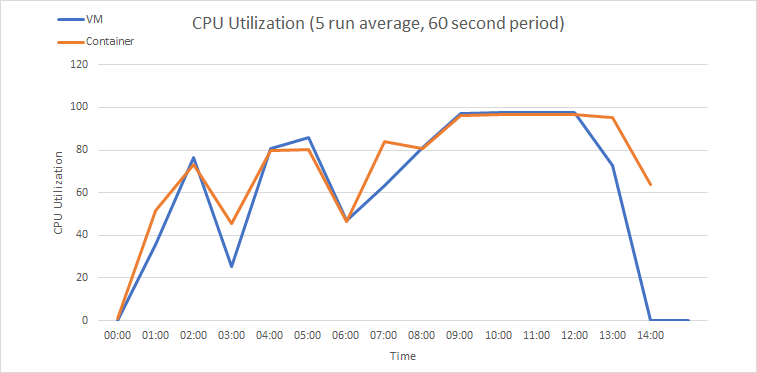
\includegraphics[scale=0.3]{gbmperf_cpu}
  \captionof{figure}{gbmperf CPU Utilzation}
  \label{CPU}
\end{minipage}%
\begin{minipage}{.5\textwidth}
  \centering
  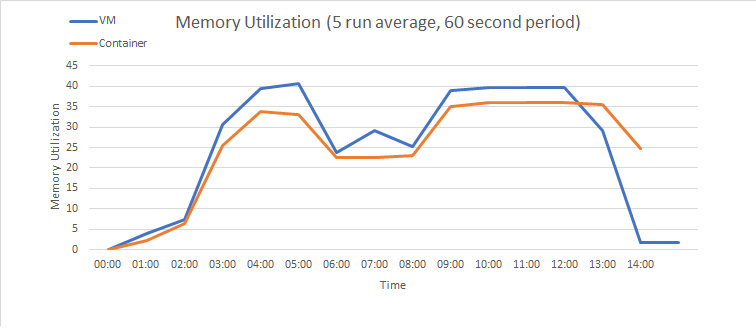
\includegraphics[scale=0.3]{gbmperf_memory}
  \captionof{figure}{gbmperf Memory Utilization}
  \label{Memory}
\end{minipage}
\end{figure}

In the case of RUBiS, each VM and container allocated 1 CPU with 2GB of memory and the benchmark was run for three times. Like gbmperf, CPU and memory utilization was averaged and graphed. Since the benchmark runs longer than gbmperf, we set the period to 5 minutes for the CloudWatch-dump data. Figures 1 and 2 show the results obtained.

Comparing the utilizations, it seems that ECS uses both more memory and more CPU when running the tests. In general, the RUBiS workload requires little CPU and memory, and only uses around 20\% and 30\% of memory on average in EC2 and ECS respectively.

\begin{figure}
\centering
\begin{minipage}{.5\textwidth}
  \centering
  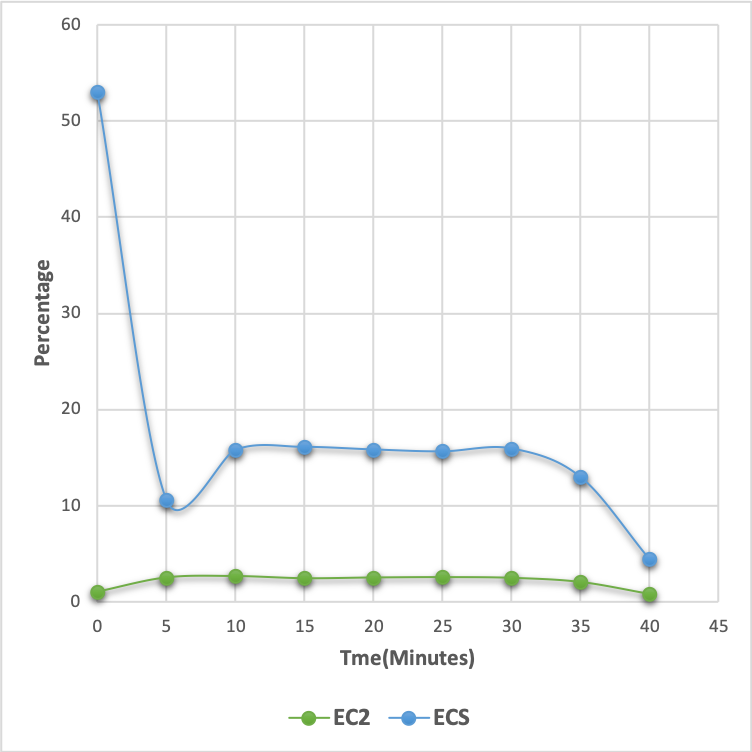
\includegraphics[scale=0.4]{CPU_rubis}
  \captionof{figure}{RUBiS CPU Utilzation}
  \label{CPU}
\end{minipage}%
\begin{minipage}{.5\textwidth}
  \centering
  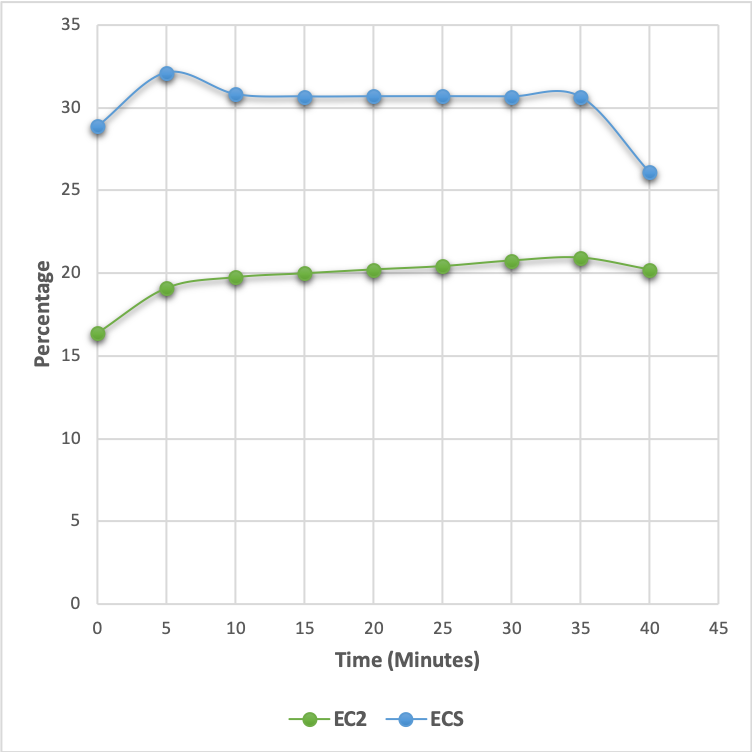
\includegraphics[scale=0.4]{Memory_rubis}
  \captionof{figure}{RUBiS Memory Utilization}
  \label{Memory}
\end{minipage}
\end{figure}

RUBiS uses an HTTP workload, where the system will continuously make HTTP requests over 40 minutes. The RUBiS benchmark itself provides results like the number of requests made for different pages of the RUBiS auction site, and also provides a summary which includes the metrics like total requests made and average requests made per second. 


\begin{center}
\captionof{table}{ECS \& EC2 Summary} 

 \begin{tabular}{||c c c ||} 
 \hline
 Instance & Number of requests & Average throughput  \\ [0.5ex] 
 \hline\hline
 ECS & 389165 & 161 req/s  \\ 
 \hline
 EC2 & 34971 & 14 req/s \\ [1ex] 
 \hline
\end{tabular}
\end{center}

The number of requests made when the workload is ran on ECS is quite larger (about 12x) than the requests made with EC2. We think that the overhead for the VM is much higher than for ECS. However, the CPU usage and memory is not bottlenecked as we observed from the usage graphs, and we speculate that there is a bottleneck in the VM somewhere else, which we'll try to find during the next phase.

\section{Unfinished Work}

The main work to complete is a second round of benchmarking and results. This involves installing the benchmarks in both VM and Docker images, running the benchmarks multiple times, and then compiling and polishing the results for presenting. The bulk of time will likely come from building the images and summarizing the results.

After comparing benchmark results, we would like to explore reasons why differences exist, or confirm that they don't, using tools such as sysbench. This will involve profiling the CPU, memory, and disk of the VMs and containers, then comparing the results.

\section{Major Barriers}

So far no major barriers have been blocking us, however certain parts proved challenging. Installing RUBiS and getting it to run was difficult due to lack of documentation and the number of services it depends on to run. We needed to install MySQL, Apache, Java, and more into a single container and automate the setup.

Additionally, to download metric data from AWS involved using a 3rd party utility that required modifications to get the correct fidelity of data. Instrumentation to the EC2 instances was also required to log CPU and memory.

\hspace{16pt}

[1] https://github.com/szilard/GBM-perf

[2] https://github.com/mogproject/cloudwatch-dump


\end{document}
